
\section{CG experimental results}

This section describes the results using the column generation approach described
in this chapter and denoted \name~here after.


%All the experiments were conducted on available RocketFuel topologies \cite{rocketfuel}
%for reproducibility.
%Their characteristics are described in Table \ref{table:topos}.
We use Repetita \cite{repetita} to run all the other solvers: DefoCP \cite{defo,hartert2015solving},
Bhatia \cite{bhatia} and SRLS \cite{steven}.
We reuse the demand matrices generated for Repetita \cite{repetita}.
For each topology, they generated 5 demand matrices through the gravity model
described in \cite{gravitymodel}.
Demands were normalized so that MCF can merely force all link loads to be below or equal to 90\%.
The number of demands ranges from 7482 to 98910.
% This load is likely not reachable because MCF is a relaxation of the SRTE problem.
% MCF enables demands to be split arbitrarily and does not put a limit on the number of segments.
% 
% \begin{table}
% 	\centering
% 	\caption{Dataset summary}
% 	\label{table:topos}
% 	\begin{tabular}{|l|l|l|l|}
% 		\hline
% 		\textbf{ID} & \textbf{\# nodes} & \textbf{\# links} & \textbf{\# demands}\\
% 		\hline
% 		rf1221 & 104 & 302 & 10712 \\
% 		\hline
% 		rf1239 & 315 & 1944 & 98910 \\
% 		\hline
% 		rf1755 & 87 & 322 & 7482 \\
% 		\hline
% 		rf3257 & 161 & 656 & 25760 \\
% 		\hline
% 		rf3967 & 79 & 294 & 6162 \\
% 		\hline
% 		rf6461 & 138 & 744 & 18906 \\
% 		\hline
% 	\end{tabular}
% \end{table}

% All our experiments are easily reproducible\footnote{The code of our solver will be available at \url{https://github.com/<hidden-url>} (available from TCP chairs)}.
% Our experiments were run on a computer with 32 CPUs at 2.60GHz, 128GB of RAM and Java 1.8 JVM.
% During our experiments, \name~did not actually need 128GB of RAM but it is able to take advantage of the 32 CPUs
% thanks to the multithreading of the pricing computation.
% We used the same version of Gurobi \cite{gurobi}, v8.0, for all the solvers.

\subsection{Near-optimum evaluation}

\textbf{CG4SR provides a better lower bound for TE over SR than MCF.} Traditionally, the value of an optimal
MCF solution is used as a lower bound for
minimum maximum link utilisation that one can achieve for routing a traffic matrix. However, as mentioned
above, this bound is unrealistic as MCF is oblivious to SR. Figure \ref{fig:optimum_lowerbound} studies the quality of the lower
bound provided by \name~ compared to MCF.
The load predicted by MCF is always of about 90\% because the demand matrices of Repetita \cite{repetita}
were generated artificially to be at this value.
However, \name~shows that it is strictly impossible to escape network congestion for 5 demand matrices.
Moreover, the difference between \name~ and MCF lower bounds can be as high as 15\% in the predicted maximal load.
Increasing the number of segments does not get \name~lower bound much closer to the MCF.
%\todo{Do not vary the segment limit for lower bound in the figure ?}

\begin{figure}
\begin{center}
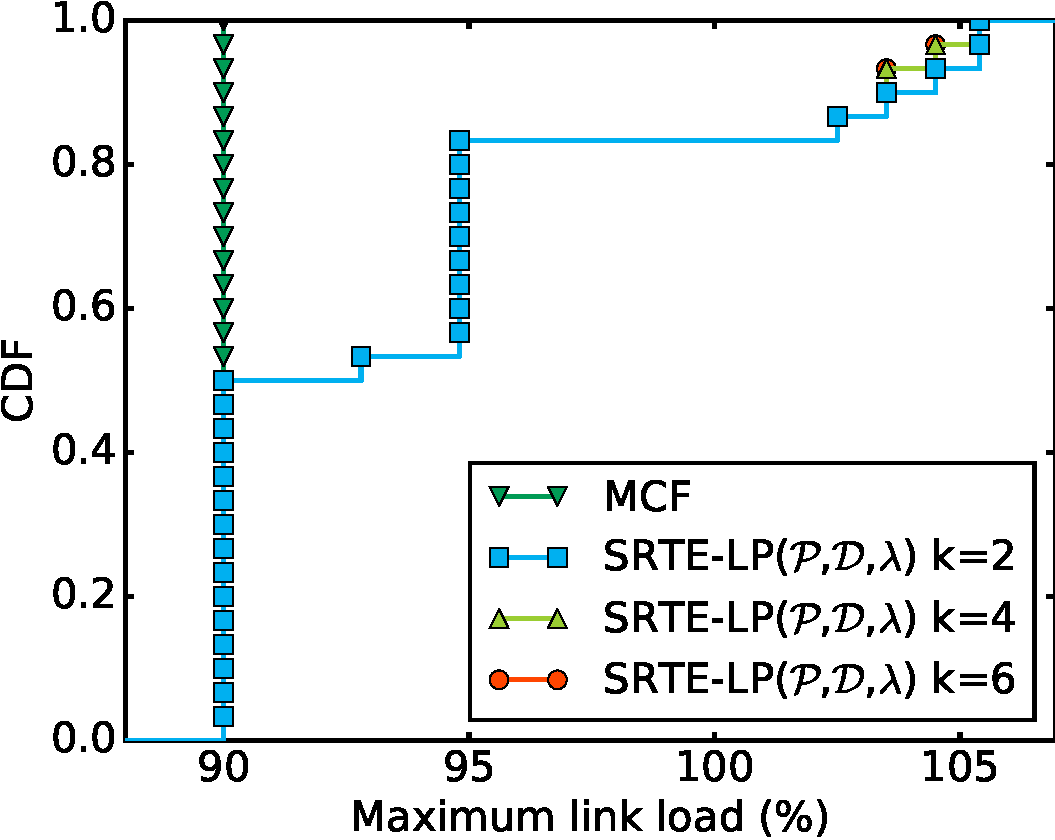
\includegraphics[width=0.8\textwidth]{images/solver_lower_bound_seg_cmp.2016RocketFuelUCL.cdfs.pdf}
\end{center}
\caption{Lower bound}
\label{fig:optimum_lowerbound}
\end{figure}


%The first question to answer is how near \name~really is to the optimality.
\textbf{CG4SR provides solutions whose maximum load is at most 4\% more than the optimal solution.} 
We ran \name~without enabling adjacency segments and without time limit.
The experiment was repeated with limits of 2, 4 and 6 segments
to observe the impact of the segment limit on the quality of the solution.
Figure \ref{fig:optimum:gap} shows CDFs of the gap (in percents)
between the \name~upper and lower bounds
on all the 30 instances (i.e., 5 demand matrices for each of the 6 topologies)
and increasing the limit on the number of segments.
This gap is the maximum distance to the actual optimum.
We can see that increasing the limit from 2 to 4 segments impacts
the quality of the solution while increasing the limit from 4 to 6 has little impact.
Paths with 4 or 6 segments add more flexibility than paths with 2 segments
to SRTE-UTIL-ILP.
We can see that this gap is most of the time below 1\% of the load and at worst 4\% of the load
if 4 segments are allowed.


\begin{figure}
\begin{center}
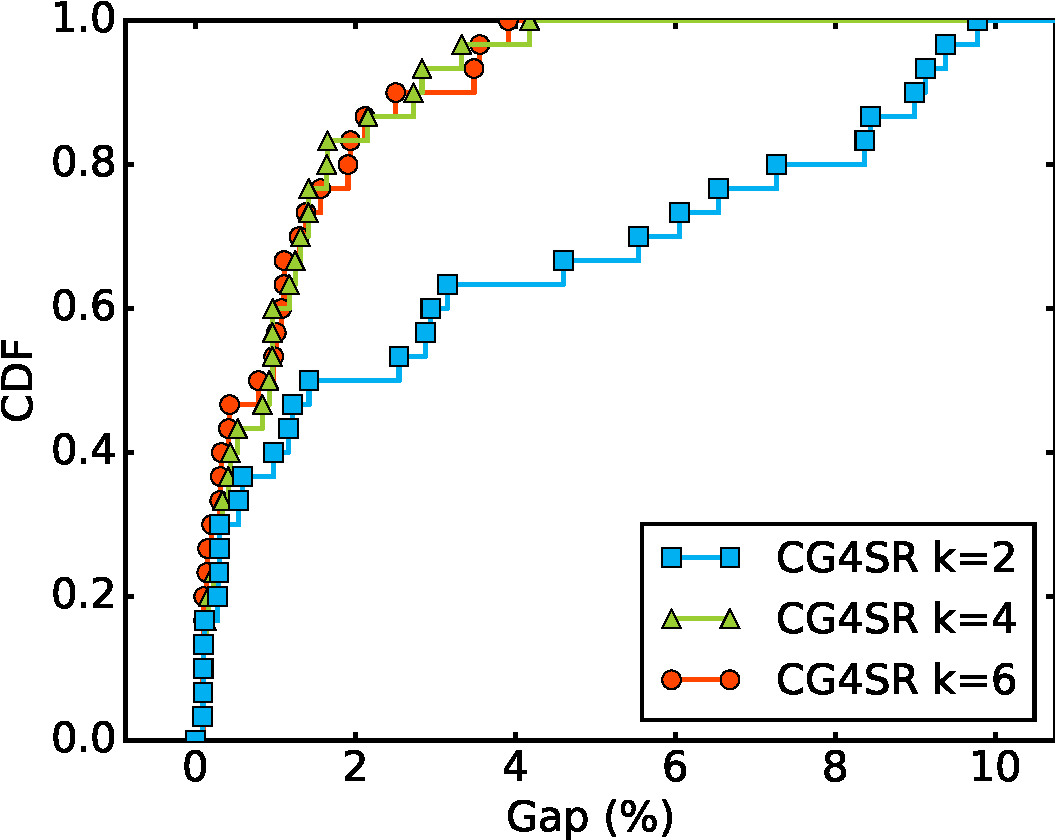
\includegraphics[width=0.8\textwidth]{images/solver_gap_optim_seg_cmp.2016RocketFuelUCL.cdfs.pdf}
\end{center}
\caption{Gap}
\label{fig:optimum:gap}
\end{figure}


\textbf{CG4SR is more efficient than Bhatia and MCF.} 
We compared the speed of \name~to Bhatia, MCF and MCFP. MCFP is an efficient variant of MCF that is only able to
compute the optimal value of MCF, not the actual routing paths.
%All these solvers provide guarantee on their final solutions.
Figure \ref{fig:optimum:time} describes how fast the different solvers can find
their best solution.
During these runs, the limit on the number of generated paths
at each column generation iteration, \textit{maxp} in Algorithm \ref{algo:iterate}, is fixed to 10.
This figure shows a CDF of the execution time on the different topologies and
demand matrices for \name, Bhatia and MCF.
Because Bhatia only allows two segments, \name~is also limited to two segments in this figure.
MCF is the slowest one and it runs out of memory for all the demand matrices
of the largest topology despite the 120GB available.
Bhatia only considers paths that can be expressed with two segments.
This significantly reduces the problem size and Bhatia can always get an answer.
\name~can run with any number of two segments because of the lazy generation of the paths.
And this is so effective than we are actually faster than Bhatia with a two-segment limit.

Figure \ref{fig:optimum:time} also shows that the MCFP variant of MCF
can actually compute the optimal value of the MCF quicker than \name.
But, as mentioned above, MCFP only provides the maximum link
utilisation of the MCF formulation but not a set of paths satisfying it. Hence, in practice, MCFP can
only be used to provide lower bounds which, as we showed in Figure \ref{fig:optimum:gap}, are worse
than the ones provided by our algorithm.

%while the optimal value is the same as the MCF formulation,
%we cannot extract paths that satisfy its optimal value.
%Moreover,there is no guarantee that the MCFP solution is actually reachable,
%nor how far from the real optimal it could be.

\begin{figure}
\begin{center}
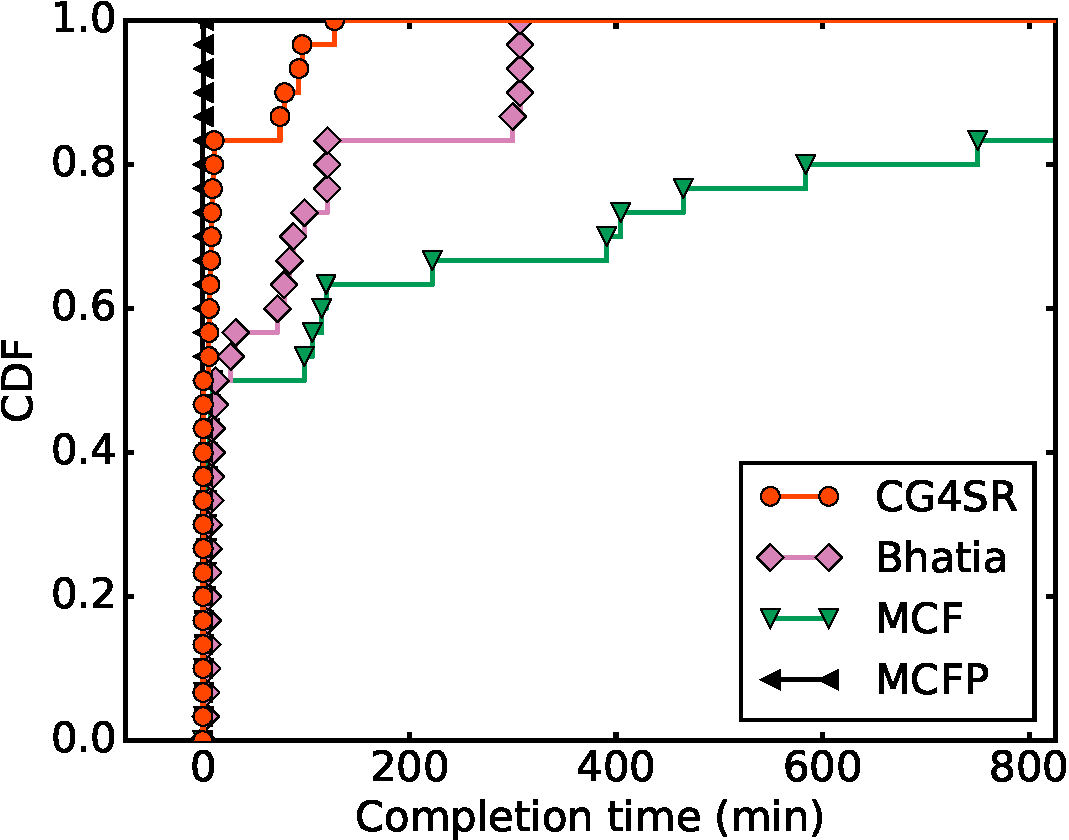
\includegraphics[width=0.8\textwidth]{images/solver_exec_times_inf-2.2016RocketFuelUCL.cdfs.pdf}
\end{center}
\caption{Execution time (\name~is limited to two segments)}
\label{fig:optimum:time}
\end{figure}


\textbf{CG4SR scales better than MCF and Bhatia.}
Our model has fewer variables than the MCF and Bhatia formulations.
The size of our model is the number of paths that were generated.
The size of MCF considers how much of each demand can be placed on each edge.
Therefore, the number of variables is the number of edges multiplied by the number of demands.
Bhatia considers for each demand, two segments through a single node of the graph.
Its number of variables is thus the number of nodes multiplied by the number of demands.
We observe that \name~is more scalable
because it considers at worst 60 times fewer possibilities than Bhatia
and 200 times fewer than MCF. This explains why \name~is faster than Bhatia and MCF.
This difference does not change significantly when varying the limit on the number of segments.
As can be seen in Figure \ref{fig:size:colgen},
the number of generated columns seems to grow linearly with the number of demands.
Given that the restricted path set is initialized with all the direct paths for every demand,
the path-finding process (Algo \ref{algo:iterate}) only creates a limited number
of additional paths to reach optimality.
This also explains why the column generation approach is so efficient in practice, as it only needs to solve the linear program
with a number of variables only slightly above the number of demands.
%\todo{Pierre: Enough dots for conclusions ?}

\begin{figure}
	\centering
	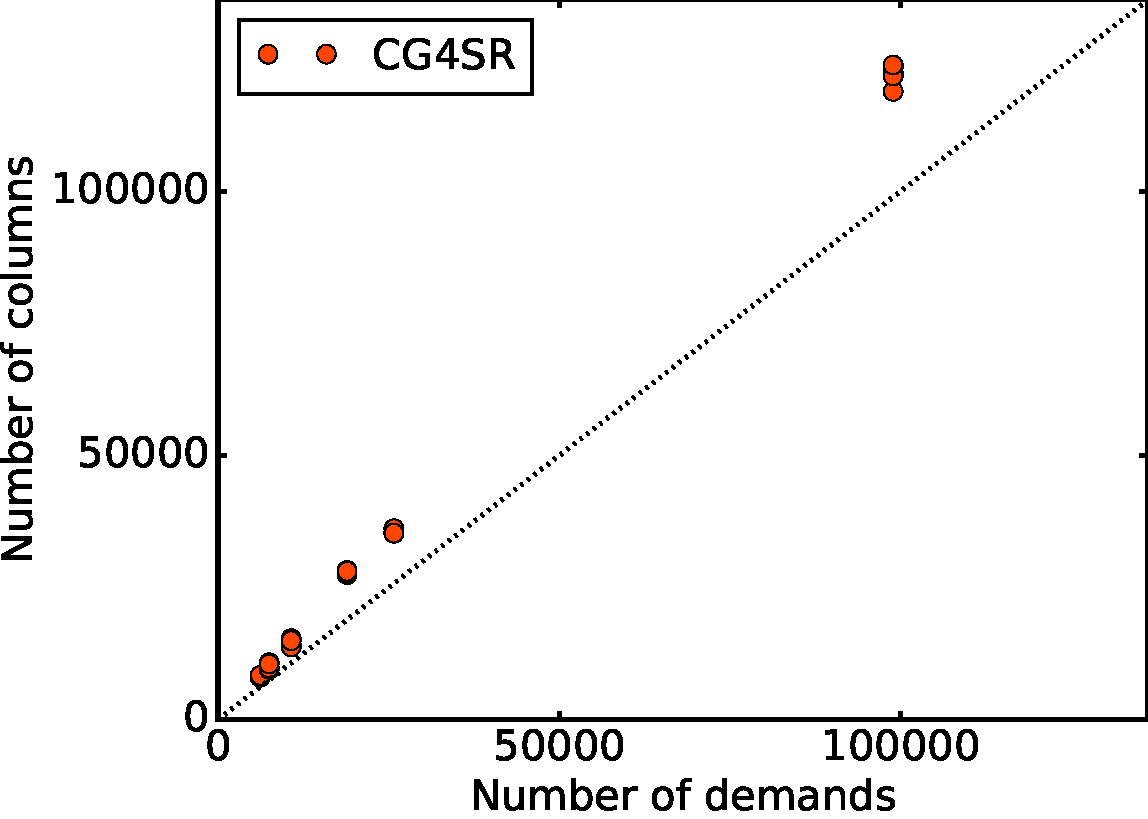
\includegraphics[width=0.8\textwidth]{images/solver_columns_over_demands_inf-6.2016RocketFuelUCL.pdf}
	\caption{Number of generated columns over the size of the demand matrices}
	\label{fig:size:colgen}
\end{figure}


\subsection{Any-time behavior}

The previous section shows that we can produce quality solutions with illimited time budget.
This section evaluates the quality of \name~solutions over time.
We compare \name~ to the heuristic approaches DEFO, SRLS and also to Bhatia.

\textbf{CG4SR finds good solution even if only allowed to run for a short amout of time.}
Figures \ref{fig:anytime:1min}, \ref{fig:anytime:5min}
and \ref{fig:anytime:10min} show, for each of the cited solvers, a CDF of the gap
to the SRTE-LP solution for the cited solvers after,
respectively 1 minute, 5 minutes and 10 minutes.
During these runs, the \textit{maxp} parameter (see Algorithm \ref{algo:iterate}) of \name, is fixed to 10.
The limit of segments is set to 5, except for Bhatia which limits itself to 1.
The quality of a solution is the difference between its current solution and the \name~lower bound
that was computed without time limit and the same limit on the number of segments.

We see that we are always faster than Bhatia even with limited time spans.
SRLS and DEFO are heuristic approaches and therefore are able to quickly find good solutions.
Figure \ref{fig:anytime:1min} shows that \name~ is already comparable to SRLS and better than DEFO
for half of the instances after 1 minute.
We see that DEFO initially finds better solutions but \name~catches up for most of instances
by increasing the timeout in Figure \ref{fig:anytime:5min} and Figure \ref{fig:anytime:10min}.
The largest instance is not yet solved after 10 minutes and that explains why DEFO is still better.

\begin{figure}
\begin{center}
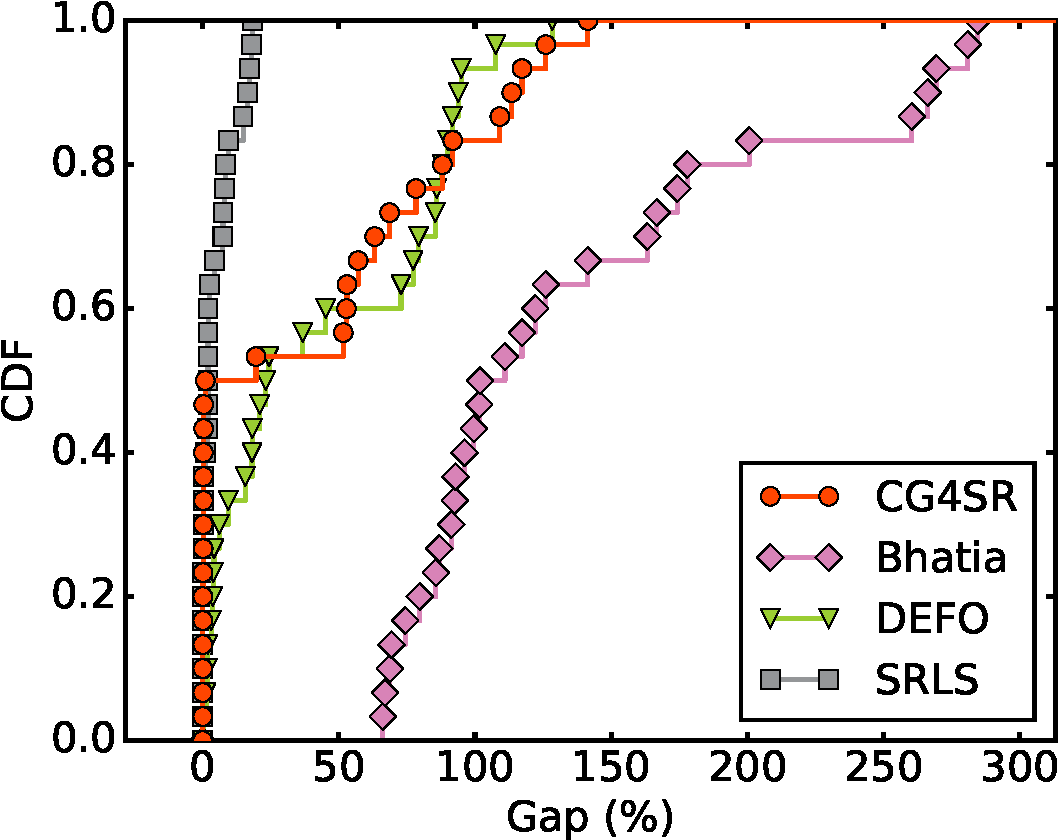
\includegraphics[width=0.8\textwidth]{images/solver_gap_optim_60-6.2016RocketFuelUCL.cdfs.pdf}
\caption{Timeout at 1 minute}
\label{fig:anytime:1min}
\end{center}
\end{figure}

\begin{figure}
\begin{center}
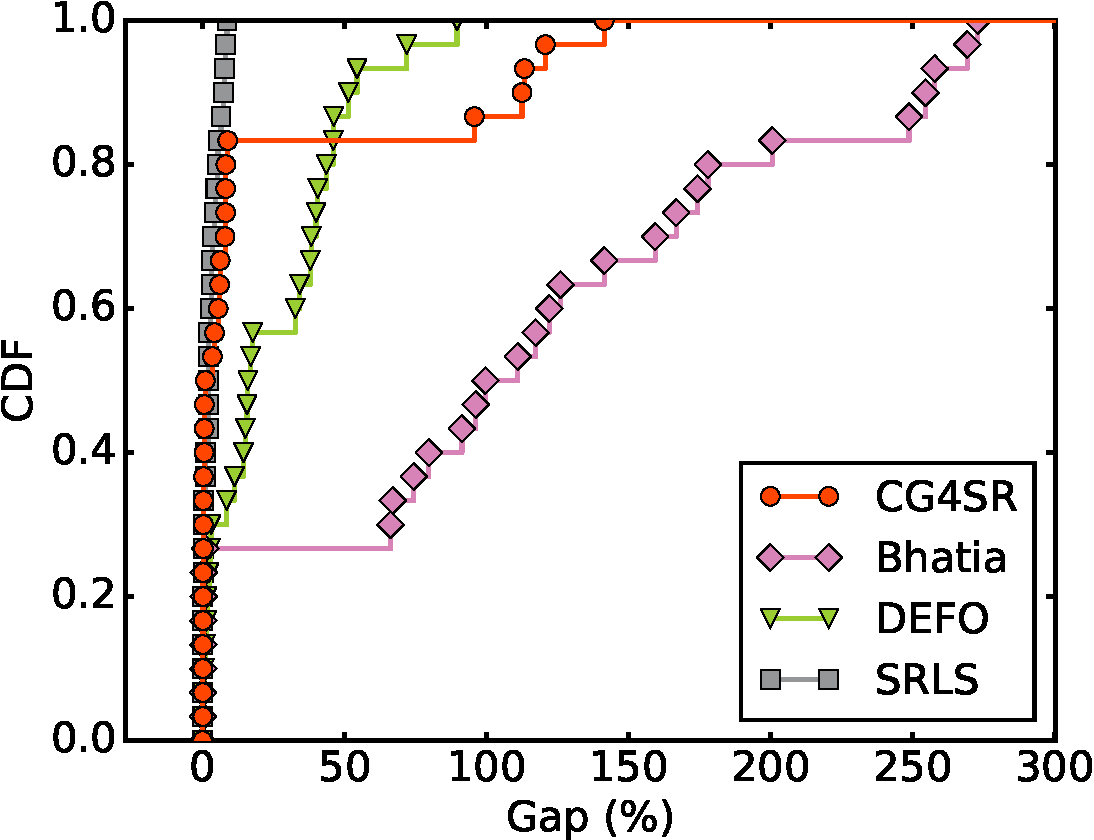
\includegraphics[width=0.8\textwidth]{images/solver_gap_optim_300-6.2016RocketFuelUCL.cdfs.pdf}
\caption{Timeout at 5 minutes}
\label{fig:anytime:5min}
\end{center}
\end{figure}

\begin{figure}
\begin{center}
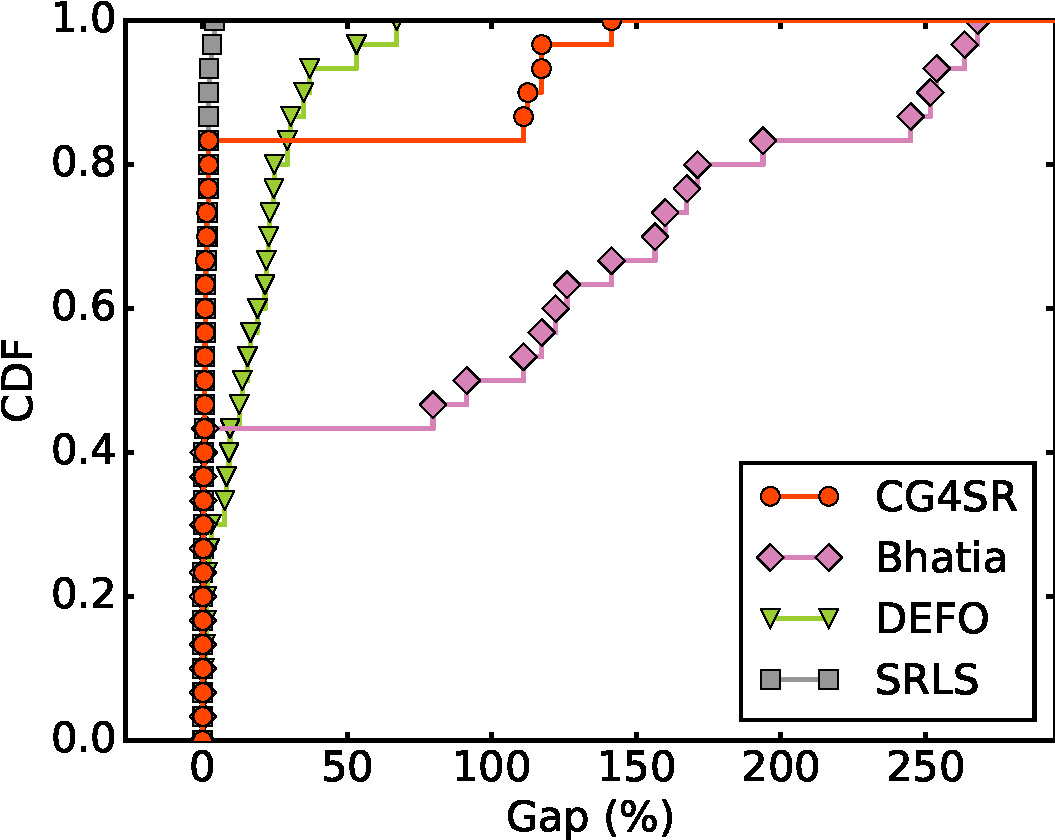
\includegraphics[width=0.8\textwidth]{images/solver_gap_optim_600-6.2016RocketFuelUCL.cdfs.pdf}
\caption{Timeout at 10 minutes}
\label{fig:anytime:10min}
\end{center}
\end{figure}


\textbf{CG4SR is more robust than SRTE over different sets of demands.}
SRLS produces good results but however this solution is based on local search and can be stuck in a local optimum.
We did not observe it on the demand matrices generated by the gravity model.
The demand volumes are generally much lower than link capacities.
This also means that there are many possible ways to reach good solutions,
even if the best solution is hard to find.
The gravity model is a good match to the Traffic Engineering problem in ISPs
but demand volumes are likely higher in inter-datacenter communication \cite{b4}.
This also means that there are fewer good solutions.
We generated one additional demand matrix for each RocketFuel topology
with a low number of large demands requiring 95\% of the bandwidth available
between their source and destination.
Figure \ref{fig:anytime:srlsdefense} shows a CDF of the quality of the solution with
a time limit of 10 minutes and a limit of six segments as in Figure \ref{fig:anytime:10min}.
These results confirm that SRLS can be worse than \name~when fewer good solutions are available.

\begin{figure}
	\centering
	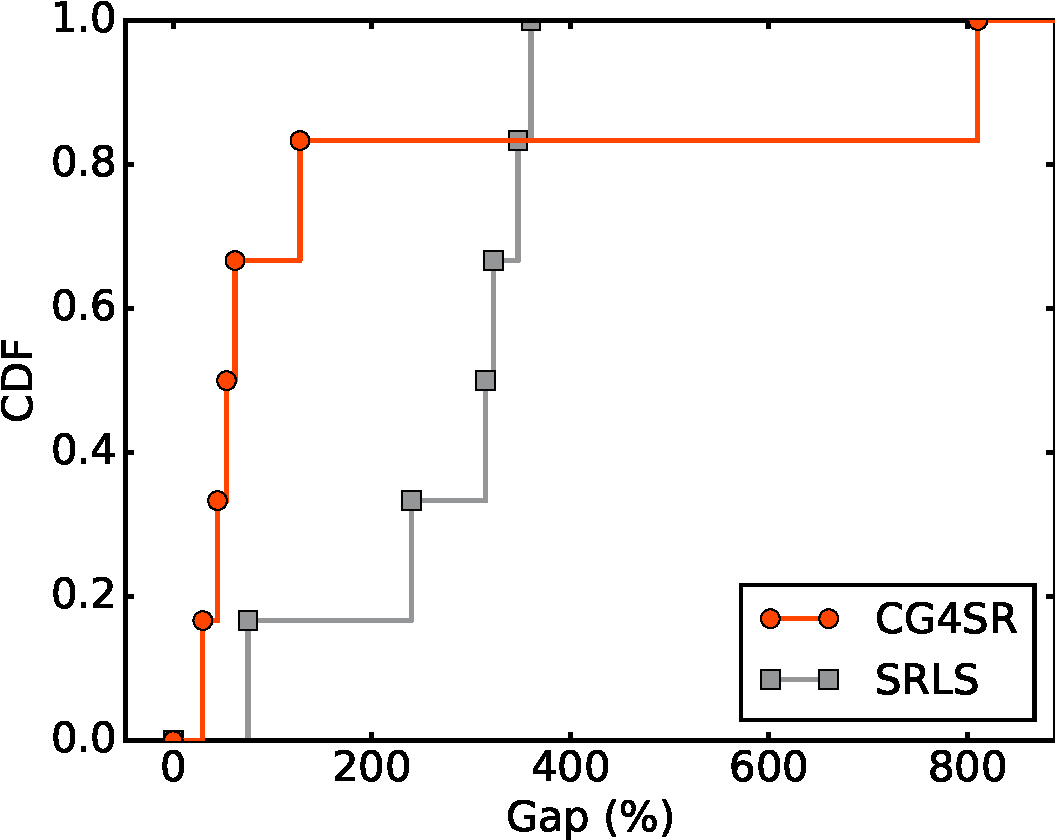
\includegraphics[width=0.8\textwidth]{images/solver_gap_optim_600-6.2016RocketFuelUCL_datacenter.cdfs.pdf}
	\caption{Gaps between $SRTE-LP(\P,\D,\lambda)$ and SRLS or \name~after 10 min with a limit of 6 segments}
	\label{fig:anytime:srlsdefense}
\end{figure}

%\textbf{CG4SR avoids to use SR on too many paths.}
%The gap is not the only criteria of the quality of a solution.
%Since the encoded stack of Segment Routing labels takes space into each packet,
%they take bandwidth resources to be transmitted.
%That is, if two solutions have the same gap to \name~lower bound,
%it's best to choose the one with fewer paths with at least two segments.
%Figure \ref{fig:anytime:10min:detours} shows how many paths need at least two segments to reach the solutions
%in Figure \ref{fig:anytime:10min}.
%We see that Bhatia finds solutions mostly without any segment but they have bad gaps,
%meaning that Bhatia did not have the time to find segments.
%When its gaps are good, it uses 2 segments on almost all the paths.
%\name~cannot find good segments for 5 instances (the demand matrices of the largest topology).
%Yet, for all the other instances, for a similar gap, it detours fewer demands than SRLS.
%DEFO detours fewer paths than \name~ but cannot always reach similar gaps.

%\begin{figure}
%	\centering
%	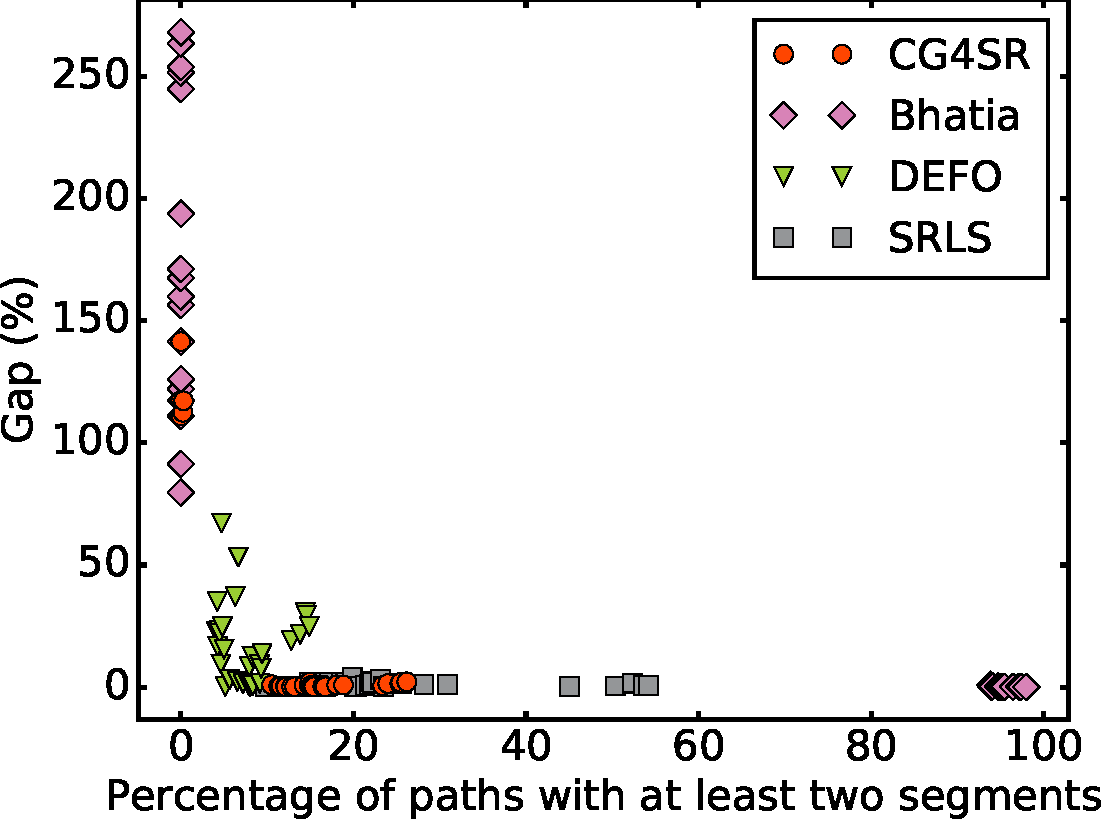
\includegraphics[width=0.3\textwidth]{images/solver_detoured_paths_600-6.2016RocketFuelUCL.pareto.pdf}
%	\caption{Gaps over the percentage of paths with at least two segments. We fixed the time limit to 10 minutes and the limit of segments to 6.}
%	\label{fig:anytime:10min:detours}
%\end{figure}

\subsection{Adjacency segment benefits}

\textbf{Adjacency segments are important in TE and CG4SR is the first to use them.}
\name~is the first SR traffic engineering model to support adjacency segments.
We evaluate the benefits of adjacency segments on the inter-datacenter network topology of OVH
in Europe (described in \cite{scmon}).
This topology has more parallel links than RocketFuel topologies and
thus, the OVH topology can really benefit from adjacency segments.
We do not have access to the link weights and capacities of OVH.
Therefore, for each link bundle we set the capacity of half of the links to some value and the other
half to half of that value. This simulates the link upgrades on the network. For pairs of
nodes with a single link between them, we set the capacity to be ten times bigger.
Five demand matrices were generated for the OVH topology with the gravity model \cite{gravitymodel}.

Figure \ref{fig:adjacency:upperbound} shows CDFs of the gap (in percents)
between the \name~upper and lower bounds over the demand matrices of the OVH topology.
We do not limit the execution time and we limit the number of segments to 4.
This means that we allow at most one detour through a specific link
because one segment is needed for the destination and a link detour costs two segments.
Even allowing only one link detour halves the load of the maximally loaded link
because it utilizes better the parallel links of this topology.

\begin{figure}
	\centering
	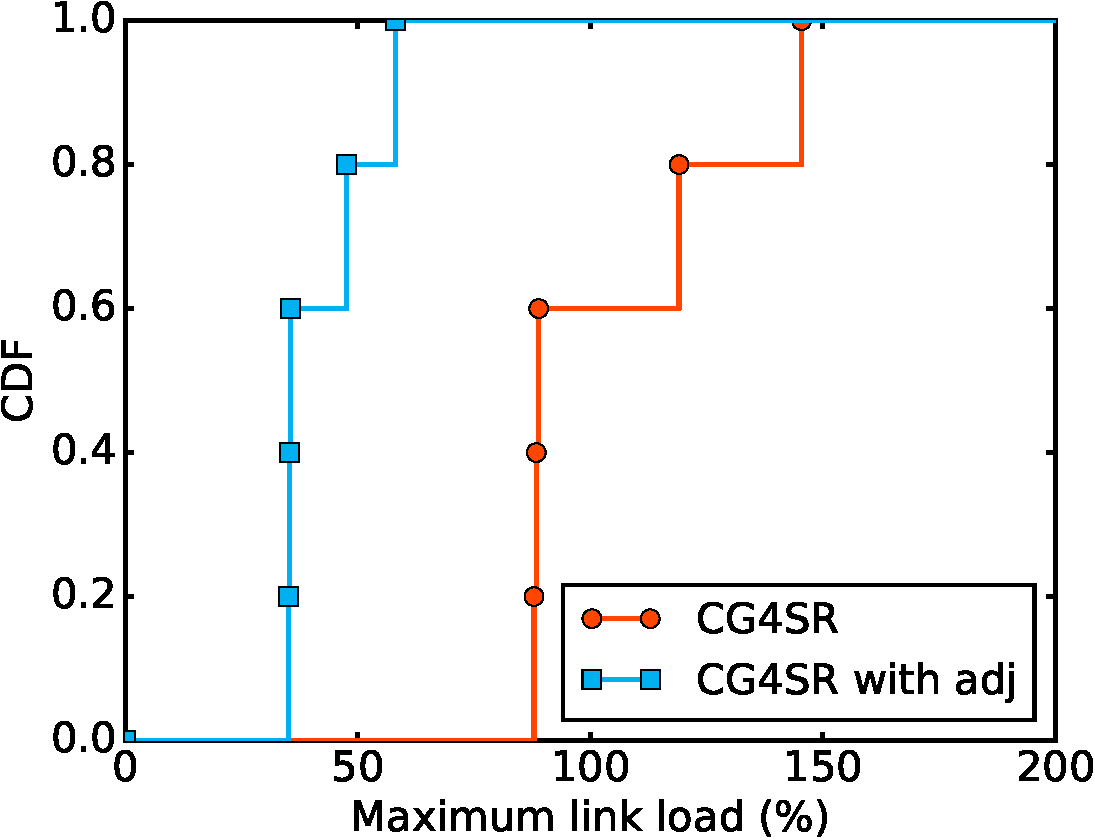
\includegraphics[width=0.8\textwidth]{images/solver_adj_upper_bound.OVH_paper.cdfs.pdf}
	\caption{The \name~solutions with or without adjacency segments. The limit of segments is fixed to 4.}
	\label{fig:adjacency:upperbound}
\end{figure}

